\documentclass[11pt]{article}
\usepackage[latin1]{inputenc}
\usepackage{a4wide}
\usepackage{amsmath}
\usepackage{amsfonts}
\usepackage{amssymb}
\usepackage{graphicx}
\usepackage{enumerate}
\usepackage{epstopdf}
\usepackage{float}
\usepackage{multicol}
\usepackage{hyperref}
\epstopdfsetup{outdir=./images/}
\usepackage{subcaption}

\title{Natural Computing, Assignment 6}
\author{Dennis Verheijden - s4455770 \and Pauline Lauron - s1016609 \and Joost Besseling - s4796799}
\begin{document}
\maketitle

\section*{Note}
After a lot of struggling to get the source code up and running using Matlab, compiling the binaries necessary, we managed to get it to run. 

However, we quickly stumbled upon a multitude of errors. We believe they were due to incompatible code, where the code was written for $<$MATLAB 2018a. For example, the function \texttt{svmtrain} was used, which has been deprecated.

We tried to circumvent this issue by using an older version of MATLAB, 2015b. Here the functions were not deprecated, however we did not manage to successfully compile the necessary binaries. As a last resort, we copied the source code for these deprecated functions, which ultimately worked. However, we then got presented with the error that we could not predict multi-class problems with this function. Which is weird, because the original implementation was built to handle multi-class problems.

We also had to fix some errors where the input for certain functions were incorrect, due to typing errors. Such as for the function \texttt{idivide}.

The latter could be fixed, such that we could successfully run Ad-REM. However we did not get CORAL to run, due to many deprecations.

We then tried to implement CORAL ourselves in python. We implemented it as described in the provided paper, but the results are not as expected. Where, if we did not use CORAL but instead use both raw datasets, the results were better than when we applied CORAL.

\section{Using Zero Target Data}
\subsection{Ad-REM}
\begin{itemize}
	\item[VGG:] 0.8931
	\item[SURF:] 0.4283
\end{itemize}

This difference might be accounted to the number of features that are created for each method. The VGG creates 4096 features, most having some meaningful values (i.e. not-sparse). Whereas SURF outputs only 800 sparse integer-values.

\subsection{CORAL}
\begin{itemize}
	\item[VGG:] ---
	\item[SURF:] ---
\end{itemize}

\section{Experiment}

\subsection{SURF}
For the experiment we randomly selected a percentage $p$ of the labeled target-data for each class. Each experiment was repeated 10 times. The results may be seen in figure \ref{fig:adrem_results_surf}. What we can see from this boxplot is that using more labeled data increases the accuracy. Which is to be expected, following the ``more data is better'' ideology. 

\begin{figure}[H]
	\centering
	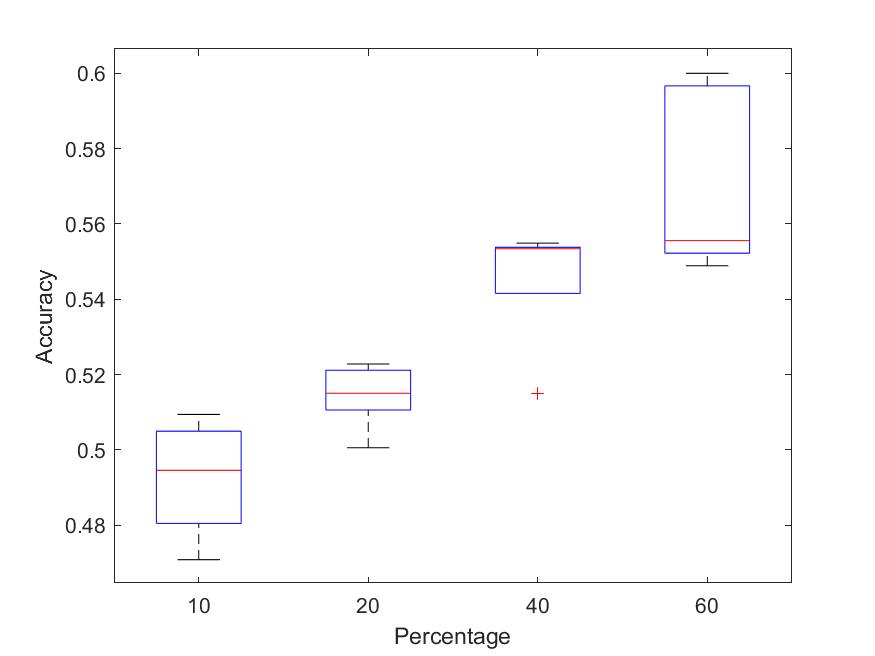
\includegraphics[width=0.7\textwidth]{images/adrem_results_surf.png}
	\caption{Boxplot of the results for Ad-REM on the SURF dataset.}
	\label{fig:adrem_results_surf}
\end{figure}

\subsection{VGG}
We also do the same experimentation with the VGG dataset. We can conclude the same that using more labeled data increases the accuracy. Which is to be expected, following the ``more data is better'' ideology. 

\begin{figure}[H]
	\centering
	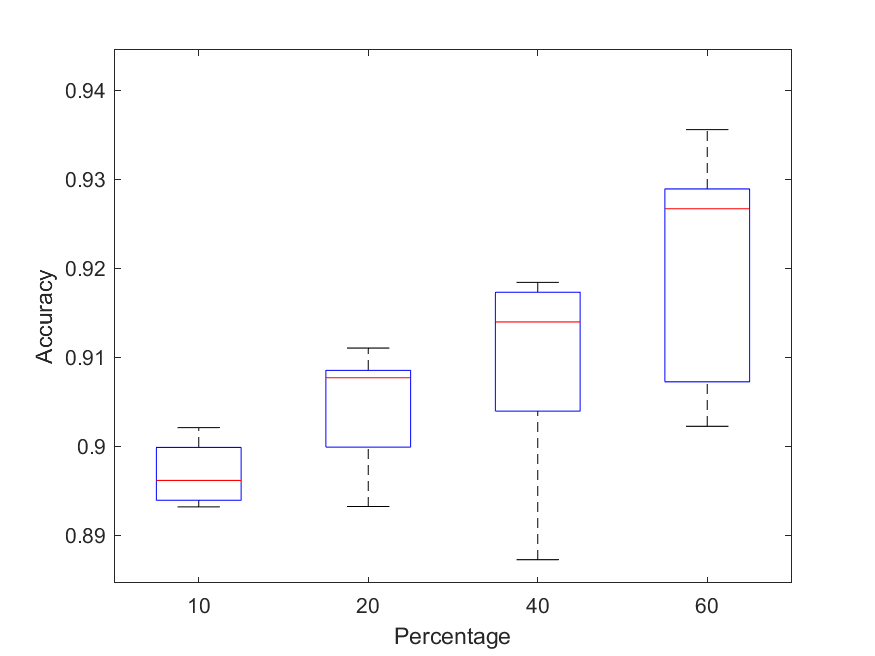
\includegraphics[width=0.7\textwidth]{images/adrem_results_vgg.png}
	\caption{Boxplot of the results for Ad-REM on the VGG  dataset.}
	\label{fig:adrem_results_vgg}
\end{figure}
\end{document}